%%
\subsection{突発天体の研究} \label{transients.s1.introduction}
%%
\subsubsection{はじめに}

\paragraph{呼称}
電波帯域における突発天体は広く知られており、その起源は超新星爆発やガンマ線バーストの電波残光、活動銀河核フレアなど多種多様である。
その呼び方も、フレアと呼ばれたりバーストと呼ばれたり、場合によってはフラッシュなどと呼ばれることもあるが、それらを全て含む包括的な呼び方としては「突発的な」という意味を表すトランジェント (transient) という単語が用いられる。
特に電波帯域における突発天体・突発現象は{\bf 電波トランジェント} (radio transients) と総称され、例えば超新星爆発も電波トランジェントのひとつといえる。
呼び方に取り決めはないが、既知天体の増光現象はフレアと呼び、それよりも大幅な増光をする爆発的現象をバースト、その他の起源のわからない現象に対しては包括的にトランジェントと呼んでしまうことが多い。
また数秒以下の短いタイムスケールの変動に対してはパルスと呼ぶことも多い。

\paragraph{突発天体と変動天体}
光度変動を繰り返す天体、つまり変動天体も突発天体と見なすことがある。
周期的または非周期的に光度変動を起こす天体があったとき、その光度が大きく常に観測できていれば変動天体と見なされるが、一方で本質的には変動していても、光度が小さすぎるために一時的にしか観測できなければ突発天体と見なされる。
例えば後述する rotating radio transients (RRATs) という散発的なパルサーは、そのような例だと考えられる。
変動天体と突発天体を区別することはさし当たって重要ではないため、それらを同一視し、例えばパルサーも突発天体の枠に含んで議論する。

\paragraph{既知の突発天体と未知の突発天体}
たいていの突発天体は電磁波の波長によらず発見され、ある波長域で観測された突発天体は、他の波長域においても対応天体が観測される。
例えば超新星爆発は主に光学領域で発見されるが、それらは電波やX線でも増光が観測され、場合によってはガンマ線バーストが同時観測されることもある。
さらには光子のみならず、他の素粒子の一つであるニュートリノが観測されることもある。
しかしその一方で、他波長では対応天体が見つからなかったり、対応天体が見つかってもその放射機構が未知であるような、起源のわからない突発天体も多い。
このように宇宙には、既知の突発天体だけでなく、未知の突発天体が数多く隠れている。

\paragraph{SKAを用いた突発天体研究の方向性}
この現状を踏まえてSKAは、既知の現象に対してはその高い性能を生かして緻密な観測を行い、現象について従来より詳細な情報を得ることで、その「物理の解明」に寄与する。
また未知の現象に対しては、観測システムの柔軟性とデータ解析システムの多様性を実現することで、まだ実施されたことのないような観測や解析による探査を行い、科学にとって最も重要な「未知の発見」を目指す。

%%
\subsubsection{突発天体の分類}
%%
突発天体・変動天体の分類方法は2通りあり、(1) 地球からの見え方にもとづく分類法と、(2) 放射源での物理にもとづいた分類法がある。
前者 (1) の分類法では、\Tabref{tb:frail-classification}のように突発天体をその位置と光度変動のタイムスケールによって分類する\citep{2012ApJ...747...70F}。
この分類はかなり大雑把だが、発見に必要となる観測方法を示唆する。
観測方法は、光度変動のタイムスケールによって大きく異なり、数秒以下の短時間変動のものは時系列データから直接検出され、それ以上の長時間変動のものはイメージング観測による画像データから検出されることが多い。
\begin{table}
	\centering
	\caption{電波帯域における突発・変動天体の分類 (1)}\label{tb:frail-classification}
	\begin{tabular}{|c|c|c|}
		\hline
		&
		{\gt 短時間変動} &
		{\gt 長時間変動} \\ \hline

		{\gt 銀河系外}	&
		Fast Radio Bursts &
		超新星爆発$^\dagger$, 活動銀河核など \\ \hline
		
		{\gt 銀河系内}	&
		パルサーなど &
		恒星フレア, メーザーバーストなど \\ \hline		
	\end{tabular}
	\begin{tablenotes}
	この分類法では、地球から突発天体を観測したときに、その天体が天の川銀河の外にあるか、中にあるか、またその光度が数秒以下という短時間で変動するか、それ以上の長時間にわたって変動するか、というように4分類している。
	\end{tablenotes}
	\begin{tablecomments}{\dagger}
	超新星爆発は銀河系内でも起こりうるが、観測される超新星のほぼ全てが系外のものである。
	人類によって観測された系内超新星は 1604 年の SN~1604 が最後であり、それ以降に系内超新星は見つかっていない。
	\end{tablecomments}
\end{table}%

一方で (2) の分類法では、放射された電波に干渉性があるかないか (コヒーレントかインコヒーレントか) によって突発現象を2分類する。
その分類を詳細に図示したものが\Figref{fig:transients.phasespace}である (Cordes et al., in prep)。
この図は突発・変動現象をプロットした相空間であり、各プロットは一つの天体、あるいは現象を示す。
コヒーレント放射による突発現象は図の白地の領域にプロットされ、インコヒーレント放射による突発現象は水色の領域にプロットされる。
同種の天体や放射機構が同じ現象はこの図の中で同じ領域を占有し、例えば図のやや左下にパルサーが群集しておりコヒーレント放射であることがわかる。
この図が突発天体研究において最も重要な図であり、次節で詳述することにする。
\begin{figure}
	\centering
	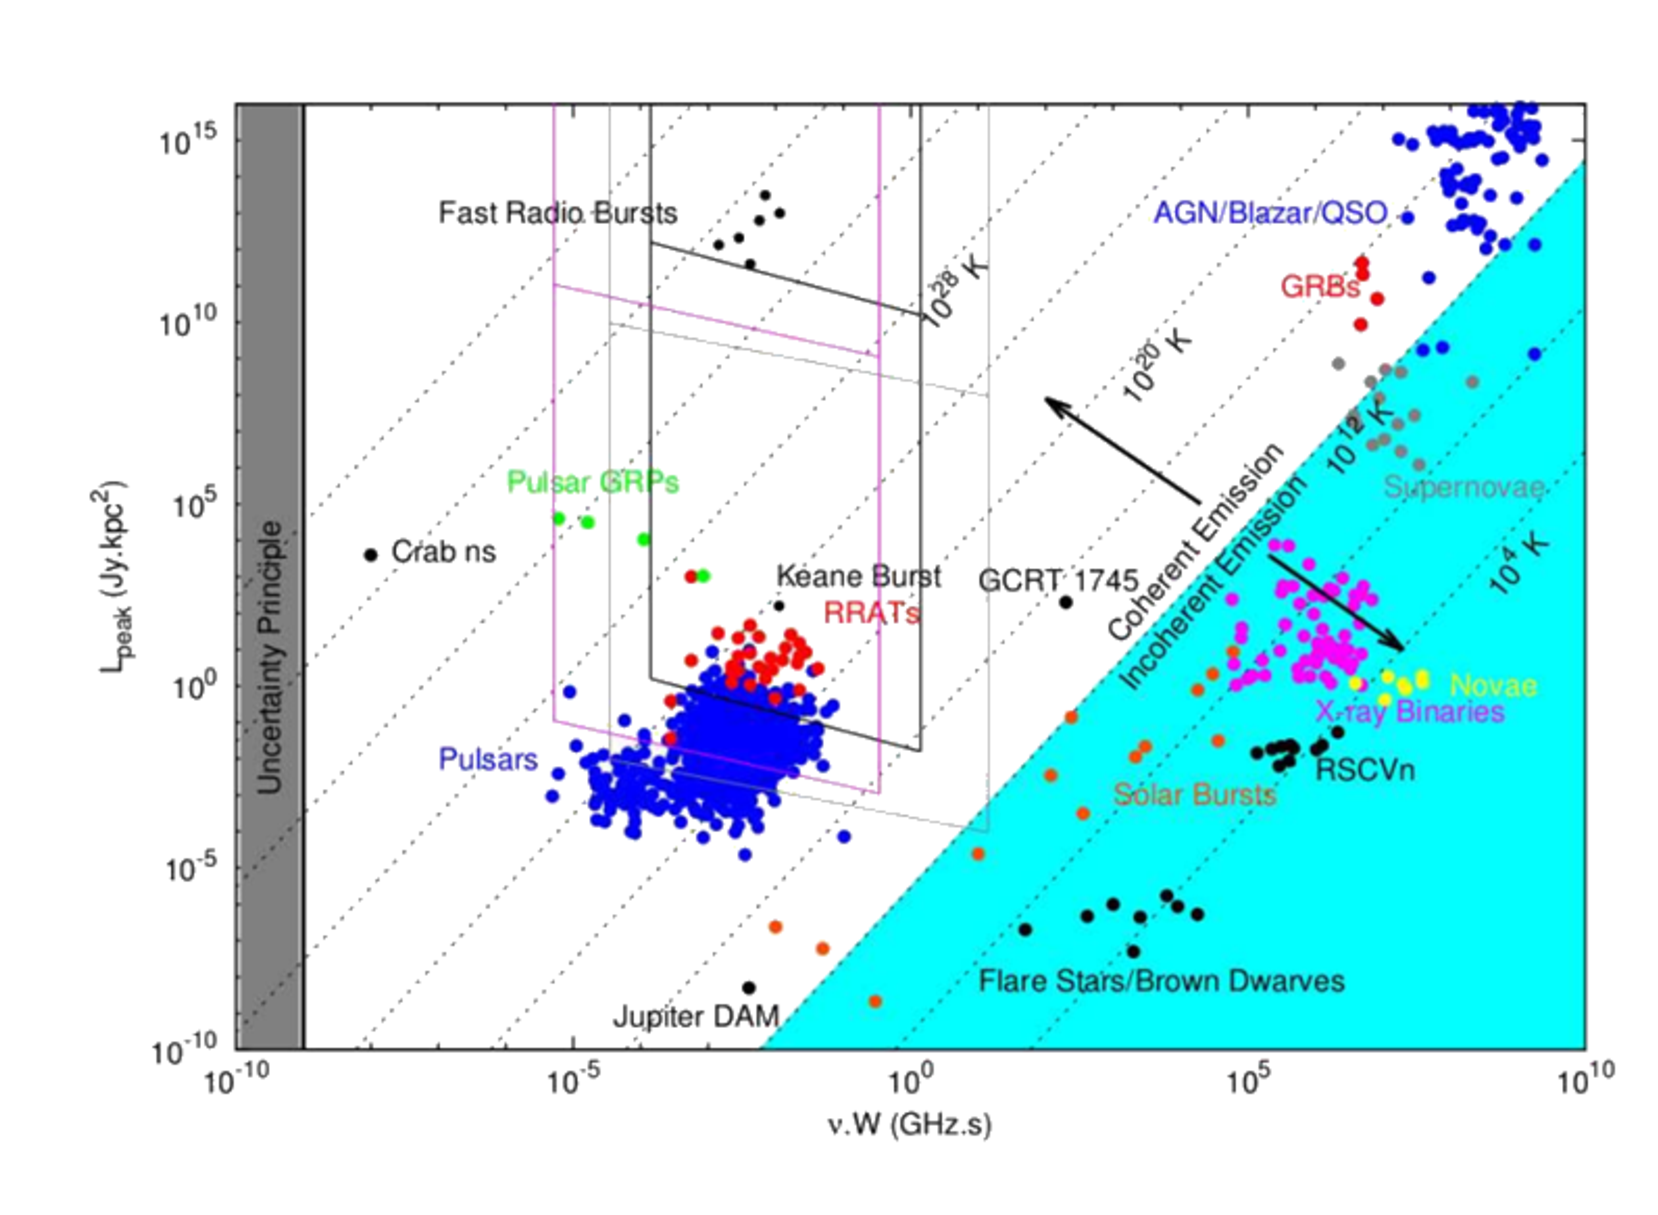
\includegraphics[width=0.9\textwidth]{transients/transients.phasespace.eps}
	\caption{突発・変動現象の相空間 (Cordes et al., in prep)。縦軸は光度変動の極大値、横軸はその変動のタイムスケールを意味し、各プロットは現象を表す。}
	\label{fig:transients.phasespace}
\end{figure}%
%コヒーレントな放射をする突発現象としては、例えばパルサーからのパルスやFRBが挙げられ、光度変動のタイムスケールは数秒以下と短い。
%変動している時間が短いため、それらは時系列の生データを解析することによって発見される。
%一方インコヒーレントな放射をする突発現象としては、例えばX線連星 (中性子星と恒星の連星など) からのバーストや超新星爆発が挙げられ、それらの多くは光度変動のタイムスケールが比較的長い。
%それらの変動は短くとも数日以上続き、たいていの場合数か月以上続くため、イメージング観測による画像データの中から発見されることが多い。

%%
\subsubsection{突発天体・変動天体の相空間}
%%
種々の突発天体をプロットした\Figref{fig:transients.phasespace}は、天体の光度$SD^2$とその変動の継続時間$W$が
\begin{align}
	SD^2 = 2 \pi k_\text{B} T (\nu W)^2, \quad \text{i.e.,} \quad
	\left( \frac{S}{\text{Jy}} \right) \left( \frac{D}{\text{kpc}} \right)^2 = 9.11 \times 10^{-18} \times
		\left( \frac{T}{\text{K}} \right) \left( \frac{\nu}{\text{GHz}} \cdot \frac{W}{\text{s}} \right)^2,
	\label{eq:transients.phasespace}
\end{align}
で関係付けられることに基づいている。
ここで$S$はフラックス密度、$D$は天体までの距離、$k_\text{B}$はボルツマン定数、$T$は輝度温度、$\nu$は観測周波数、$W$は変動の継続時間を表す。
%\footnote{電波の輝度温度とは、その電波が黒体から放射されたと見なしたときの、その黒体のもつ熱力学温度に等しい温度のこと。}
\Figref{fig:transients.phasespace}では縦軸に$SD^2~(=L_\text{peak})$、横軸に$\nu W$を取っており、複数の右上がりの直線は異なる温度$T$における\Eqref{eq:transients.phasespace}を図示したものである。

ここで\Eqref{eq:transients.phasespace}は以下のように導かれる。
レイリー・ジーンズ近似のもとで、電波天体の放射強度は $I_\nu \simeq 2\nu^2 k_\text{B} T / c^2$ と与えられる。
ここで$c$ は光速を表し、その他の量は前述のとおりである。
観測者から見た放射源の角度半径を $\theta_\text{src}$とすると、観測者の受信するフラックス密度$S$はその定義から
\begin{equation}
	S = \int_0^{2\pi} \td \phi \int_0^{\theta_\text{src}} \td \theta \sin \theta \cdot I_\nu \cos \theta
\end{equation}
で与えられる。
ここで実際の放射源の半径を $R_\text{src}$、観測者から放射源までの距離を$D$とすると、 $|\theta_\text{src}| \ll 1$であるから$\theta_\text{src} \simeq \tan \theta_\text{src} = R_\text{src} / D$と近似してよい。
また放射源の大きさ$R_\text{src}$ は変動の継続時間 $W$を用いて $R_\text{src} \simeq c W$として見積もることができるので、結局$\theta_\text{src} \simeq cW/D$と表せる。
したがってフラックス密度は
\begin{equation}
	S \simeq \pi \left( \frac{cW}{D} \right)^2 \cdot \frac{2\nu^2 k_\text{B} T}{c^2}
\end{equation}
と書け、これを変形すると\Eqref{eq:transients.phasespace}を得る。
以上のようにして、変動の継続時間 $W$ はその光度 $SD^2$ と関連付けられることがわかる。
この関係は、レイリー・ジーンズ近似、 $\theta_\text{src} \simeq \tan \theta_\text{src}$および$R_\text{src} \simeq c W$という3つの妥当な近似に基づいている。

以上のように\Figref{fig:transients.phasespace}は\Eqref{eq:transients.phasespace}に基づいた相空間を表しているが、その相空間は放射の輝度温度によって2つの領域 (白色と水色の領域) に分けられる。
地球で観測できる電波放射現象の多くは、インコヒーレントなシンクロトロン放射からなる。
しかしシンクロトロン電波の光子に電子が衝突する逆コンプトン効果によって、その光子はX線のエネルギーにまで叩き上げられ、結果的に電波の強度は制限されるという現象が起こる。
その制限された電波強度は、輝度温度にして$10^{12}~\text{K}$であり、もしある天体の輝度温度がその値を超えていた場合、その放射はコヒーレント放射かドップラー増幅されていることになる。
この輝度温度$10^{12}~\text{K}$の直線が、\Figref{fig:transients.phasespace}でコヒーレント放射の領域 (白色) とインコヒーレント放射の領域 (水色) を区切っている。

\Figref{fig:transients.phasespace}はすべての突発現象を網羅しているわけではないが、この相空間に広がる空白領域は、まだ発見されていない現象が数多く眠っていることを表している。
未知の現象があるということは、それを発見できれば新たな物理を開拓できる可能性があるということであり、科学はそのような未知の発見によって発展してきた。
したがって、\Figref{fig:transients.phasespace}の空白領域を埋めるような観測を積極的に行い、未知の現象を発見していくことが天文学者にとって重要な仕事となる。
その仕事を効率的に進めるには、高い感度と広い視野によって広範囲を探査することが必要であり、SKAはまさにそのような探査を可能とする。

